\documentclass[12pt]{article}

% Packages
\usepackage[margin=0.6in]{geometry}
%\usepackage[dvipdfm]{graphicx} 

\usepackage{graphicx} 
\usepackage{bmpsize}
\usepackage{amsmath}
\usepackage{float}
\usepackage[dvipsnames]{xcolor}
\usepackage{etoolbox}
\usepackage{soul}

%\usepackage{tcolorbox}
%\definecolor{block-gray}{gray}{0.85}

\pagestyle{plain}


\begin{document}

\title{Solution ark \#3.\\ Ratio and regression estimation}
\author{O\u{g}uz--Alper, Melike \& Pekarskaya, Tatsiana, Statistics Norway}
\maketitle

\section*{Exercise 1}
\textbf{\color{ForestGreen}(R code available)} The data set agsrs.csv contains information on the number of farms in 1987 for the SRS of $n = 300$ counties from the population of the $N = 3\,078$ counties in the
United States. In 1987, the United States had a total of $2\,087\,759$ farms and the total number of acres devoted to farming was $964\,470\,625$.
\begin{enumerate}
\item Plot the data.\\
\fcolorbox{black}{ForestGreen!20}{
\begin{minipage}[t]{0.97\linewidth} 
\textbf{Solution:}
We will be interested in the exercise in finding an estimated for number of acres devoted to farming in 1992. And we will use information on number of farms and acres from year 1987 to get the estimate. Thus, the plots we are interested in are the next:
\begin{figure}[H]
\begin{center}
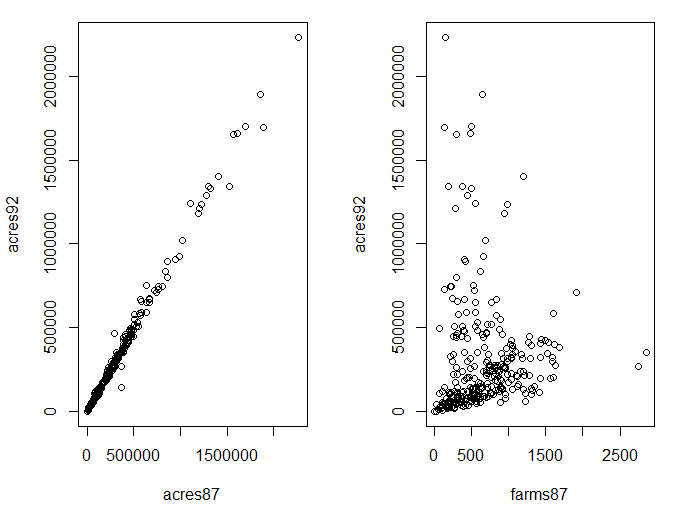
\includegraphics[scale=0.9]{Ex1_1.png}
\end{center}
\end{figure}
\end{minipage}}
\item Use ratio estimation to estimate the total number of acres devoted to farming in 1992, using the number of farms in 1987 as the auxiliary variable.\\
\fcolorbox{black}{ForestGreen!20}{
\begin{minipage}[t]{0.97\linewidth} 
\textbf{Solution:}
With ratio estimation, assuming $\bar{X}/\bar{x}\approx 1$ and knowing that $\hat{B} = \frac{\hat{t}_y}{\hat{t}_x} = \frac{\bar{y}}{\bar{x}}$, and thus using
$$\hat{t}_{y;r}=\hat{B}t_x,  \quad
\hat{V}(\hat{t}_{y;r})=N^2\, \Big(1-\frac{n}{N}\Big)\frac{s_e^2}{n}, \quad e_i=y_i-\hat{B}x_i, \quad s_e^2 = \frac{1}{n-1}\sum_{i \in s}e_i^2$$
we obtain\\
$\hat{t}_{y;r;farms87}=459.8975*2\,087\,759=960\,155\,061$\\
$\widehat{SE}(\hat{t}_{y;r;farms87})=3\,078\,\sqrt{1-\frac{300}{3\,078}}\,\frac{387\,172.3}{\sqrt{300}}=65\,364\,822$
\end{minipage}}
\item Repeat (2), using regression estimation.\\
\fcolorbox{black}{ForestGreen!20}{
\begin{minipage}[t]{0.97\linewidth} 
\textbf{Solution:}
With regression estimation, using
$$\hat{t}_{y;reg}=(\hat{B}_0+\hat{B}_1\,\bar{X})N,   \quad \hat{V}(\hat{t}_{y;reg})=N\,\Big(1-\frac{n}{N}\Big)\frac{s_e^2}{n},\quad e_i=y_i-\hat{B}_0-\hat{B}_1 x_i,$$
and $\hat{B}_0 = \bar{y} - \hat{B}_1\bar{x}, \quad \hat{B}_1 = \sum_{i \in s}(x_i - \bar{x})(y_i - \bar{y})/\sum_{i \in s}(x_i - \bar{x})^2$
we obtain
$$\hat{t}_{y;reg} = 267\,029.8*3\,078 + 47.65325*2\,087\,759=921\,406\,265$$
$$\widehat{SE}(\hat{t}_{y;reg})=3\,078\,\sqrt{1-\frac{300}{3\,078}}\,\frac{343\,938.4}{\sqrt{300}}=58\,065\,813$$

\end{minipage}}
\item Which method gives the most precision: ratio estimation with auxiliary variable
$acres87$, ratio estimation with auxiliary variable $farms87$, or regression estimation
with auxiliary variable $farms87$? Why?\\
\fcolorbox{black}{ForestGreen!20}{
\begin{minipage}[t]{0.97\linewidth} 
\textbf{Solution:}\\
First, we calculate ratio estimation with auxiliary variable $acres87$: \\ 
$\hat{t}_{y;r;acres87}=0.9866*964\,470\,625=951\,513\,191 $\\
$\widehat{SE}(\hat{t}_{y;r;acres87})=3\,078\,\sqrt{1-\frac{300}{3\,078}}\,\frac{31\,657.22}{\sqrt{300}}=5\,344\,567$\\

\begin{center}
\begin{tabular}{lccc}
Estimation &\vline &$\hat{t}$ & $\widehat{SE}(\hat{t})$ \\
\hline
SRS, $N\bar{y}$ &\vline &916 927 110& 58 169 381\\
Ratio with acres87 &\vline &951 513 191 & \hspace{0.2 cm}5 344 568\\
Ratio with farms87 &\vline &960 155 061 & 65 364 822\\
Regression with farms87 &\vline &921 406 265 & 58 065 813\\
\end{tabular}
\end{center}
Ratio estimation with $acres87$ gives the best precision. Sample correlations are given by $\rho(x_{acres87},y)=0.9958$ and $\rho(x_{farms87},y)=0.0596$. The low correlation between acres92 and farms87 explains why neither ratio nor regression estimation with farms87 does not improve precision over the SRS estimate $N\bar{y}$.

\end{minipage}}
\end{enumerate}

\section*{Exercise 2}
\textbf{\color{ForestGreen}(R code available)} The data file counties.csv contains information on land area, population, number of physicians, unemployment, and a number of other quantities for an SRS of $100$ of the
$3\,141$ counties in the United States (U.S. Census Bureau, 1994). The total land area
for the United States is $3\,536\,278$ square miles; 1993 population was estimated to be $255\,077\,536$.
\begin{enumerate}
\item Draw a histogram of the number of physicians for the $100$ counties.\\
\fcolorbox{black}{ForestGreen!20}{
\begin{minipage}[t]{0.97\linewidth} 
\textbf{Solution:}
\begin{figure}[H]
\begin{center}
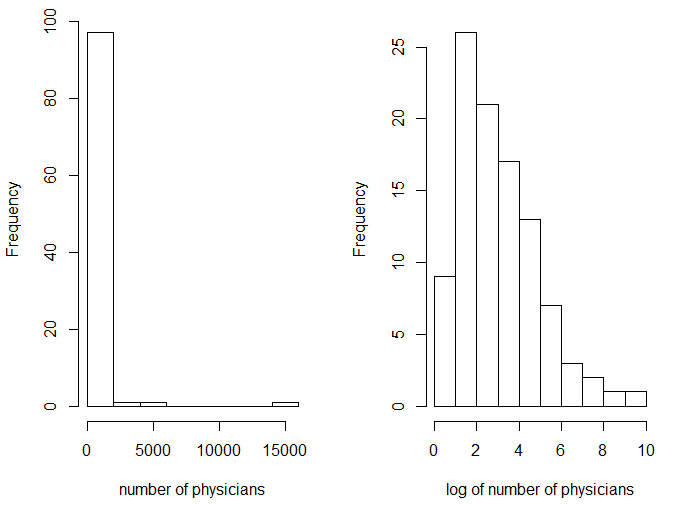
\includegraphics[scale=0.8]{Ex2_1.png}
\end{center}
\end{figure}
The histogram on the right side is the histogram of the logarithm of (the number of physicians + 1). We have a skewed distribution in both cases.
\end{minipage}}
\item Estimate the total number of physicians in the United States, along with its standard
error, using $N\bar{y}$.\\
\fcolorbox{black}{ForestGreen!20}{
\begin{minipage}[t]{0.97\linewidth} 
\textbf{Solution:}
$$N\bar{y}=933\,411, \quad \widehat{SE}(N\bar{y})=491\,982.8$$
The standard error is large in comparison to the point estimate of the total. This is a result the extreme skewness of the data, which may also lead to that $N\bar{y}$ does not follow a normal distribution. To have a normal distribution, we need, using $n_{min}=28+25\hat{\gamma}^2$ (Lohr, 2019, p.44), where $\hat{\gamma}$ is an estimate of the skewness,
$$n_{min}=28+25*8.31^2=1\,756$$

\end{minipage}}
\item Plot the number of physicians vs. population for each county. Which method do you think is more appropriate for these data: ratio estimation or regression estimation?\\
\fcolorbox{black}{ForestGreen!20}{
\begin{minipage}[t]{0.97\linewidth} 
\textbf{Solution:}
\begin{figure}[H]
\begin{center}
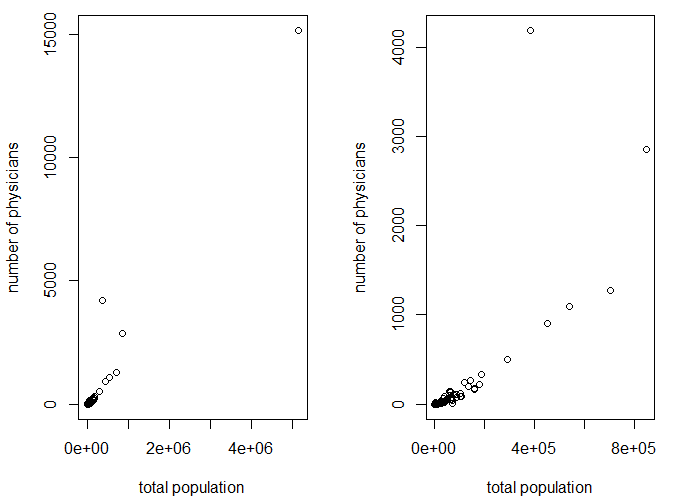
\includegraphics[scale=0.8]{Ex2_3.png}
\end{center}
\end{figure}
\vspace{-4.5mm}
The dataset used for the plots is the same with the difference that Cook county with the total number of physicians $15\,153$ is excluded in the right plot.\\
Ratio estimation may be appropriate to use since the variance seems to be increasing with increasing levels of total county population.
\end{minipage}}
\item Using the method you chose in (3), use the auxiliary variable population to estimate the total number of physicians in the United States, along with the standard error.\\
\fcolorbox{black}{ForestGreen!20}{
\begin{minipage}[t]{0.97\linewidth} 
\textbf{Solution:}
With ratio estimation, we have 
$$\hat{t}_{y;r}=0.002507*255\,077\,536=639\,506$$
Using
$$\hat{V}(\hat{t}_{y;r})=N^2\Big(1-\frac{n}{N}\Big)\Big(\frac{t_x}{N\bar{x}}\Big)^2\frac{s_e^2}{n},$$
we obtain $\widehat{SE}(\hat{t}_{y;r})=87\,885.27$. This is equivalent to what we obtain from package ``survey" in R. Without the ratio $t_x/(N\bar{x})$, we have $\widehat{SE}(\hat{t}_{y;r})=128\,275.7$.\\
With regression estimation, we have 
$$\hat{t}_{y;reg}=-54.2313*3\,141 + 0.00296*255\,077\,536=585\,871$$
Using
$$\widehat{SE}(\hat{t}_{y;reg})=3\,141*\sqrt{1-\frac{100}{3\,141}}*\frac{338.5913}{10}=104\,645$$
With the package ``survey", we obtain $\widehat{SE}(\hat{t}_{y;reg})=100\,650$, which is slightly smaller than the one given above.
\end{minipage}}

\item The “true” value for total number of physicians in the population is $532\,638$. Which method of estimation came closer? \\
\fcolorbox{black}{ForestGreen!20}{
\begin{minipage}[t]{0.97\linewidth} 
\textbf{Solution:}
Both ratio and regression estimation has provided smaller standard error, and an estimate closer to the true value comparing with SRS estimates $N\bar{y}$ and $\widehat{SE}(N\bar{y})$.
\end{minipage}}
\item Repeat parts (1)–(4) with $y=$ farm population and $x=$ land area. The “true” value for farm population is $t_y=3\,871\,583$\\
\fcolorbox{black}{ForestGreen!20}{
\begin{minipage}[t]{0.97\linewidth} 
\textbf{Solution:}
Histogram for farm population:
\begin{figure}[H]
\begin{center}
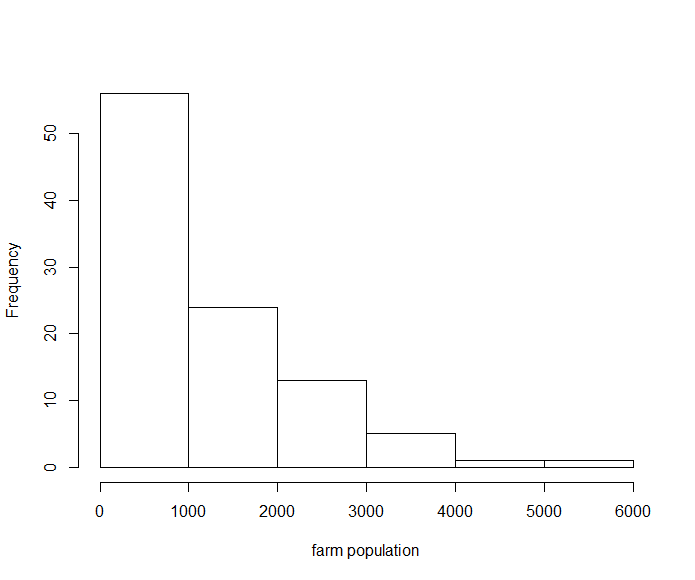
\includegraphics[scale=0.7]{Ex2_6_1.png}
\end{center}
\end{figure}
The variable farm population is skewed, but it is less skewed than the total number of physicians. \\
The SRS estimates are given by
$$N\bar{y}=3\,602\,319, \quad \widehat{SE}(N\bar{y})=329\,787$$\end{minipage}}
\\
\fcolorbox{black}{ForestGreen!20}{
\begin{minipage}[t]{0.97\linewidth}
\begin{figure}[H]
\begin{center}
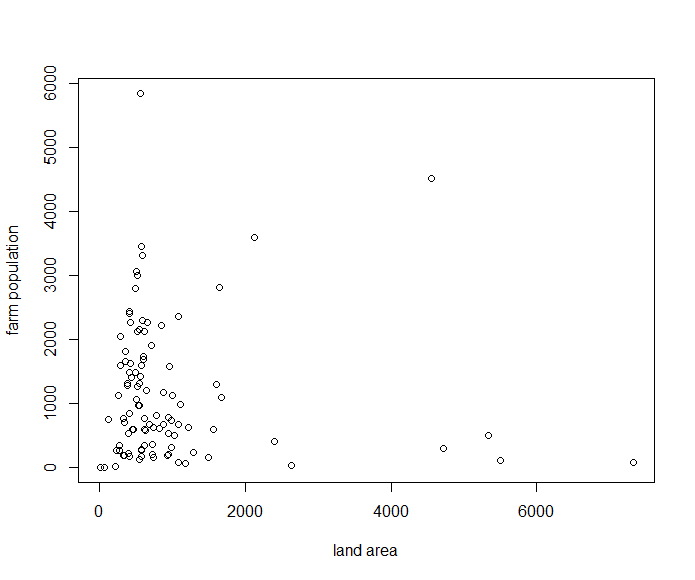
\includegraphics[scale=0.7]{Ex2_6_3.png}
\end{center}
\end{figure}
The sample correlation between farm population and land area is $\rho=-0.05811$. This means that using land area as an auxiliary information may not improve the estimation.\\
With ratio estimation, we have 
$$\hat{t}_{y;r}=1.2137*3\,536\,278=4\,292\,058$$
Using the variance estimator given in (4), we have 
$$\widehat{SE}(\hat{t}_{y;r})=668\,727.3$$ 
With regression estimation, we have 
$$\hat{t}_{y;reg}=1\,197.35 *3\,141 -0.05342*3\,536\,278=3\,571\,960$$
$$\widehat{SE}(\hat{t}_{y;reg})=3\,141*\sqrt{1-\frac{100}{3\,141}}*\frac{1\,065.263}{10}=329\,230$$
With the survey package, we obtain $\widehat{SE}(\hat{t}_{y;reg})=348\,820$, which is slightly higher than the one given above.\\
From problem statement the ``true" value of total is $t_y=3\,871\,583$. Ratio estimation has provided higher standard error, and an estimate more far away from the true value comparing with SRS estimates $N\bar{y}$ and $\widehat{SE}(N\bar{y})$. Regression estimation has neither improved the estimation. \\
\end{minipage}}
\end{enumerate}

\section*{Exercise 3}
Suppose the population consists of 4 households with total income of 210, 350, 700 and 1260(in units of kr. 1000) for households 1, 2, 3, 4 respectively. The numbers of adults in the households are 1, 1, 2 and 3 for households 1, 2, 3, 4. We take a simple random sample of size 2 for estimating the total income t ( = 2520). Consider the two estimators $\hat{t}_e = N\bar{y}_s$ and  $\hat{t}_r = t_x\frac{\bar{y}_s}{\bar{x}_s}$ where the auxiliary variable $x_i$ is the number of adults in a household i.
\begin{enumerate}
\item Find the expected value and variance (exact values) of the two estimators. Which one would you choose?\\
\fcolorbox{black}{ForestGreen!20}{
\begin{minipage}[t]{0.97\linewidth}
\textbf{Solution:}
Sampling distribution of $\hat{t}_e$ and $\hat{t}_r$:
\begin{center}
\begin{tabular}{l|cccccc}
s & (1,2) &(1,3) &(1,4) & (2,3) &(2,4) & (3,4) \\
\hline
$p(s)$ & 1/6 & 1/6 & 1/6 & 1/6 & 1/6 & 1/6\\
$\hat{t}_e$ & 1120 & 1820 & 2940 & 2100 & 3220 & 3920\\
$\hat{t}_r$ & 1960 & 2123.3 & 2572.5 & 2450 & 2817.5 & 2744\\
\end{tabular}
\end{center}
$\implies $\\
For $\hat{t}_e$ we obtain:\\
$E(\hat{t}_e) = \sum_S\hat{t}_{e;s}*p(s) = \frac{1}{6}(1120 + 1820 + \cdots + 3920) = 2520$
, which has no bias from t.\\
$V(\hat{t}_e) = E(\hat{t}_e - t)^2 = \sum_S(\hat{t}_{e;s} - 2520)^2\frac{1}{6} = 875\,466.67$\\

For ratio estimator we obtain:\\
$E(\hat{t}_r) = \sum_S\hat{t}_{r;s}*p(s) = 2444.50$, which has a small bias: slightly underestimates t.\\
$V(\hat{t}_r) = \sum_S(\hat{t}_{r;s} - 2444.50)^2\frac{1}{6} = 97192.20$\\

Comparing the two estimators we get that:\\
$SE(\hat{t}_e) = \sqrt{876466.67} = 935.67$\\
$SE(\hat{t}_r) = \sqrt{97192.20} = 311.76$\\
$\implies \hat{t}_r$ is closer, even if it is biased.\\
Note that $\sqrt{MSE(\hat{t}_r)} = \sqrt{75.5^2 + 97192.20} = 320.77$
\end{minipage}}

\item Compute the approximate 95\% confidence intervals (assuming approximate normality) based on the two estimators for all 6 possible samples. What are the exact confidence levels for the two CI procedures based on $\hat{t}_e$ and $\hat{t}_r$?\\
\fcolorbox{black}{ForestGreen!20}{
\begin{minipage}[t]{0.97\linewidth}
\textbf{Solution:}
$$SE(\hat{t}_e) = \sqrt{\hat{V}(\hat{t}_e)} = N\sqrt{(1-f)\frac{s^2}{n}}, \quad s^2 = \frac{1}{n-1}\sum_{i \in s}(y_i - \bar{y}_s)^2$$
$$SE(\hat{t}_r) = \frac{t_x}{\bar{x}}\sqrt{(1-f)\frac{s_e^2}{n}} $$
\end{minipage}}\\
\fcolorbox{black}{ForestGreen!20}{
\begin{minipage}[t]{0.97\linewidth}
\begin{center}
\begin{tabular}{l|cccc}
s & $\hat{t}_e \pm 1.96SE(\hat{t}_e)$ & Covers t? &  $\hat{t}_r \pm 1.96SE(\hat{t}_r)$  & Covers t? \\
\hline
(1,2) & $1120\pm388$ & no & $1960\pm679$ & yes\\
(1,3) & $1820\pm1358$ & yes & $2123.3\pm603$ & yes\\
(1,4) & $2940\pm2910$ & yes & $2572.5\pm764$ & yes\\
(2,3) & $2100\pm970$ & yes & $2450\pm0$ & no\\
(2,4) & $3220\pm2522$ & yes & $2817.5\pm255$ & no\\
(3,4) & $3920\pm1552$ & yes & $2744\pm326$ & yes\\
\end{tabular}
\end{center}
Not looking at that $\hat{t}_e: Pr(CI \ni t) = 5/6 = 0.83, \hat{t}_r: Pr(CI \ni t) = 4/6 = 0.67$, CI based on $\hat{t}_r$ is much more accurate and reliable.
\end{minipage}}
\end{enumerate}

\section*{Exercise 4}
\textbf{\color{ForestGreen}(R code available)} We are going to use a dataset pop\_industry.csv which contains a population of 415 companies with a given NACE (business classification code). For each company there is registered information on turnover (y) and number of employees (x). We are going to estimate turnover of the population of these 415 companies by using different estimation methods.\\
As far as sampling plan is concerned: all units with more than 50 employees, should be surveyed. For the rest – should be applied simple random sampling. The size of the sample should be such that units from the group with $> 50$ employees and $<= 50$ employees together will be 25 companies. 
\begin{enumerate}
\item Calculate estimates of total value of variable y and 95\% CI with a help of ratio ($\hat{t}_r$) and expansion ($\hat{t}_{e} = N\bar{y}$) estimators. Make sampling 10 times and fill in the table below. Compare the estimators. Which one would you prefer?\\
\begin{center}
\begin{tabular}{l||c|c|c|c}
\# sample & $\hat{t}_r$ & CI for $\hat{t}_r$ & $\hat{t}_{e}$ & CI for $\hat{t}_{e}$ \\
\hline
\hline
1&&&&\\
\hline
2&&&&\\
\hline
...&&&&\\
\hline
10&&&&\\
\end{tabular}
\end{center}

\fcolorbox{black}{ForestGreen!20}{
\begin{minipage}[t]{0.97\linewidth}
\textbf{Solution:}\\
First, we need to construct our sample:
\begin{enumerate}
\item We find all companies with more then 50 employees. There are 13 companies in the population satisfying $x > 50$.
Their total turnover is $t_{x > 50} = 1117468.$
\item Since it should be surveyed in total 25 employees, and 13 are already chosen, we take a SRS of 12 companies from the rest of population.\\
An estimate for total turnover for x $\leq$ 50 we get by:\\  
$\hat{t}_{r;x\leq50} = t_{x;x\leq50}*\frac{\bar{y}_s}{\bar{x}_s}$
\item Then ratio estimator is $$\hat{t}_r = t_{x>50} + \hat{t}_{r;x\leq50}$$.\end{enumerate}
\end{minipage}}\\
\fcolorbox{black}{ForestGreen!20}{
\begin{minipage}[t]{0.97\linewidth}
A formula for standard error to be used is:\\
$$\widehat{SE}(\hat{t}_r) = (N - n_{x>50})\sqrt{\left(1 - \frac{n_{s}}{N - n_{x>50}}\right)}\frac{\bar{x}_{x\leq50}}{\bar{x}_s}\frac{s_e}{\sqrt{n_s}},$$ where\\
$$s_e^2 = \frac{1}{n_s - 1}\sum_{i \in s}(y_i - \frac{\bar{y}_s}{\bar{x}_s}x_i)^2$$
$$95\% CI = \hat{t}_r \pm 1.96*\widehat{SE}(\hat{t}_r)$$\\
\begin{enumerate}
\setcounter{enumii}{3}
\item For expansion estimator:\\
$$\hat{t}_{e} = t_{x>50} + (N-n_{x>50})\bar{y}_s$$
$$\widehat{SE}(\hat{t}_e) = (N - n_{x>50})\sqrt{\left(1 - \frac{n_{s}}{N - n_{x>50}}\right)}\frac{s}{\sqrt{n_s}}$$
$$95\% CI = \hat{t}_e \pm 1.96*\widehat{SE}(\hat{t}_e)$$
\item We run (b)-(d) 10 times and results you can find in the table:
\end{enumerate}
\small
\begin{center}
\begin{tabular}{l||c|cc|c|cc}
\# sample & $\hat{t}_r$ & CI for $\hat{t}_r$ && $\hat{t}_{e}$ & CI for $\hat{t}_{e}$ & \\
\hline
\hline
1 & 2 786 (590) & 2 333 (013) & 3 240 (168) & 3 210 (448) & 1 733 (146) & 4 687 (749)\\
\hline
2& 3 363 (656) & 2 289 (293) & 4 438 (018) & 2 421 (992) & 1 166 (204) & 3 677 (779)\\
\hline
3& 3 309 (718) & 2 834 (031) & 3 785 (405) & 3 895 (355) & 1 116 (569) & 6 674 (141)\\
\hline
4& 3 278 (321) & 2 733 (527) & 3 823 (115) & 4 254 (877) & 2 690 (558) & 5 819 (196)\\
\hline
5& 3 159 (101) & 2 773 (913) & 3 544 (288) & 3 839 (243) & 1 118 (272) & 6 560 (213)\\
\hline
6& 3 251 (836) & 2 931 (927) & 3 571 (745) & 4 300 (940) & 1 697 (512) & 6 904 (367)\\
\hline
7& 3 288 (375) & 2 210 (133) & 4 366 (616) & 4 212 (165) &  843 (597)  & 7 580 (732)\\
\hline
8& 4 305 (811) & 1 574 (961) & 7 036 (660) & 6 504 (235) &  427 (642) & 12 580 (827)\\
\hline
9& 2 796 (453) & 2 575 (626) & 3 017 (280) & 2 269 (868) & 1 181 (599) & 3 358 (137)\\
\hline
10& 3 743 (882) & 2 197 (380) & 5 290 (384) & 3 232 (156) &  693 (740) & 5 770 (571)\\
\end{tabular}
\end{center}
Ratio estimator should be preferred to expansion estimator, since an empiric standard error of the earlier is smaller: 440 against 1195 (values are in thousands). \\
NO: The empiric standard errors were calculated by: \\
$\sqrt{V(\hat{t}_r)} \quad \sqrt{V(\hat{t}_{e})}$
\end{minipage}}
\item By taking an SRS of 25 companies from the population we get an empiric standard error for ratio estimator equal to 730 and for expansion estimator – 1589(values are in thousands) . Compare sample plans in (1) with SRS.

\fcolorbox{black}{ForestGreen!20}{
\begin{minipage}[t]{0.97\linewidth}
\textbf{Solution:}

Standard errors for both estimators in (1) were smaller than in (2): for expansion estimator 1195 against 1589, for the ratio estimator 440 against 730. It is quite obvious that a sampling plan from (1) gives a better accuracy than a standard SRS approach (2).

\end{minipage}}
\end{enumerate}
\end{document}

